\section{Understanding Recovery and Background Learning}
\label{sec:understanding-recovery}

Continuity depends on memory, but memory is not a single retrieval primitive.
Elephant Agent implements memory through five owned layers. Steps capture what
happened. Elephant State keeps one continuity line coherent. The Personal Model
keeps durable cross-line understanding. Contextual Recall retrieves support
from Steps and Facts. Background reflect decides when Step evidence should
support heavier updates.

\subsection{Conversation Search}

\texttt{tool.conversation.search} retrieves past conversation content for the
model. It answers a different question than Personal Model search: where did
this happen in the lived trail? The surface supports two modes. In
\texttt{mode=discover}, it groups matching material into copyable time ranges.
In \texttt{mode=recall}, it returns Step-level evidence from the selected
range. It reads from:

\begin{enumerate}[leftmargin=*]
  \item \textbf{SemanticIndexEntry} for vector similarity over indexed Step or
  Fact chunks;
  \item \textbf{Steps} for time-range fallback when semantic search is cold or
  empty;
  \item \textbf{Episodes} for metadata aggregation in discovery mode.
\end{enumerate}

Steps are the canonical conversation record. Query planning separates the topic
core from recall operators such as recency, current-state, historical, recap,
and verification intent. The planner handles English and CJK temporal phrases,
then retrieval applies explicit windows such as \texttt{last\_night},
\texttt{yesterday}, \texttt{last:3d}, date expressions, or ISO intervals. The
hybrid path searches each allowed scope through vector, BM25, exact keyword,
token-coverage, and n-gram signals, then reranks with a small intent-aware time
score. Semantic relevance remains primary; recency only breaks near ties or
helps when the user explicitly asks for recent material.

\subsection{Claim-Aware Personal Model Search}

When Elephant Agent needs long-term user context, it does not retrieve a generic profile
blob or nearest-neighbor memory chunk. It searches active Personal Model facts.
The retrieval unit is the fact, and source Steps remain support for the current
turn rather than truth by themselves.

\begin{figure}[t]
  \centering
  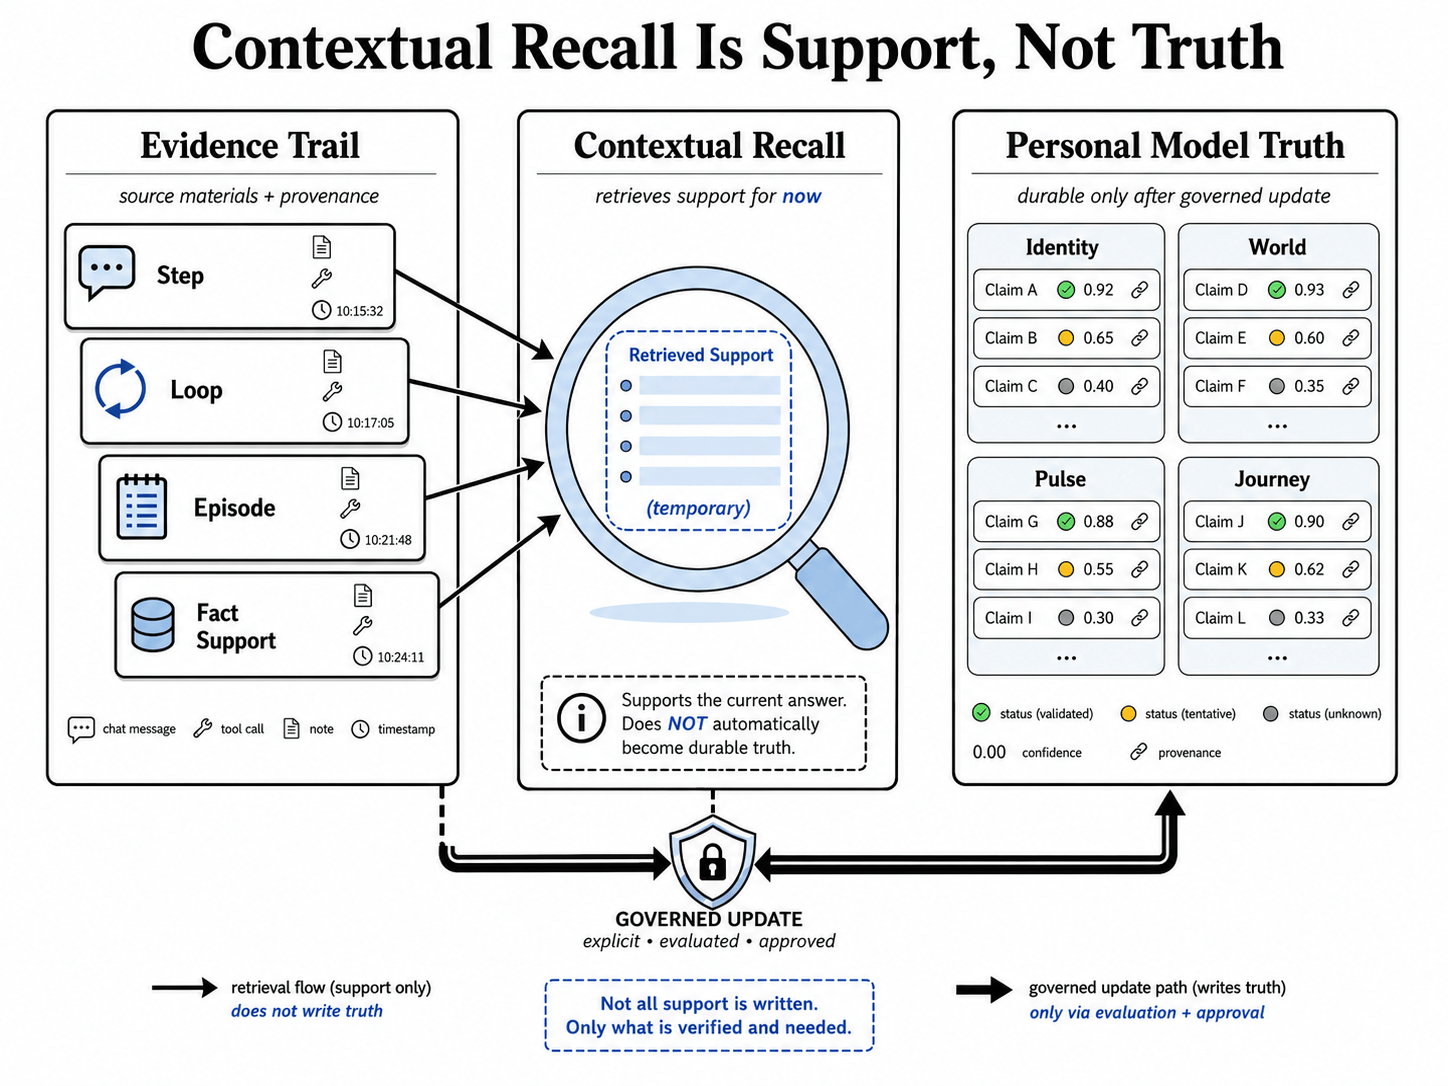
\includegraphics[width=0.9\linewidth]{../../apps/site/static/assets/resources/paper-4.png}
  \caption{Contextual Recall retrieves temporary support from the evidence
  trail, while durable Personal Model truth changes only through governed
  update paths with status, confidence, and provenance.}
  \label{fig:contextual-recall-support}
\end{figure}

The foreground search surface combines several deterministic and semantic
signals:

\begin{itemize}[leftmargin=*]
  \item topic, fact text, and source-support matches;
  \item Unicode lexical matching and CJK n-gram overlap;
  \item weak fuzzy matching for small spelling or character variation;
  \item semantic candidates from the durable index;
  \item optional translated or paraphrased query variants supplied by the model;
  \item lightweight polarity agreement or conflict for clear preference statements.
\end{itemize}

The result is thresholded. A search can return \texttt{strong\_match},
\texttt{weak\_match}, or \texttt{no\_match}. This is an important safety
property: if Elephant Agent cannot find a reliable active fact, it should expose the gap
rather than fabricate Personal Model support.

\subsection{Multilingual Hybrid Time-Aware Search}

The two search surfaces share a common retrieval posture but preserve different
truth semantics. Conversation search retrieves evidence from Steps and Episode
summaries. Personal Model search retrieves active claims. Both rely on a
multilingual hybrid search strategy:

\begin{figure}[t]
  \centering
  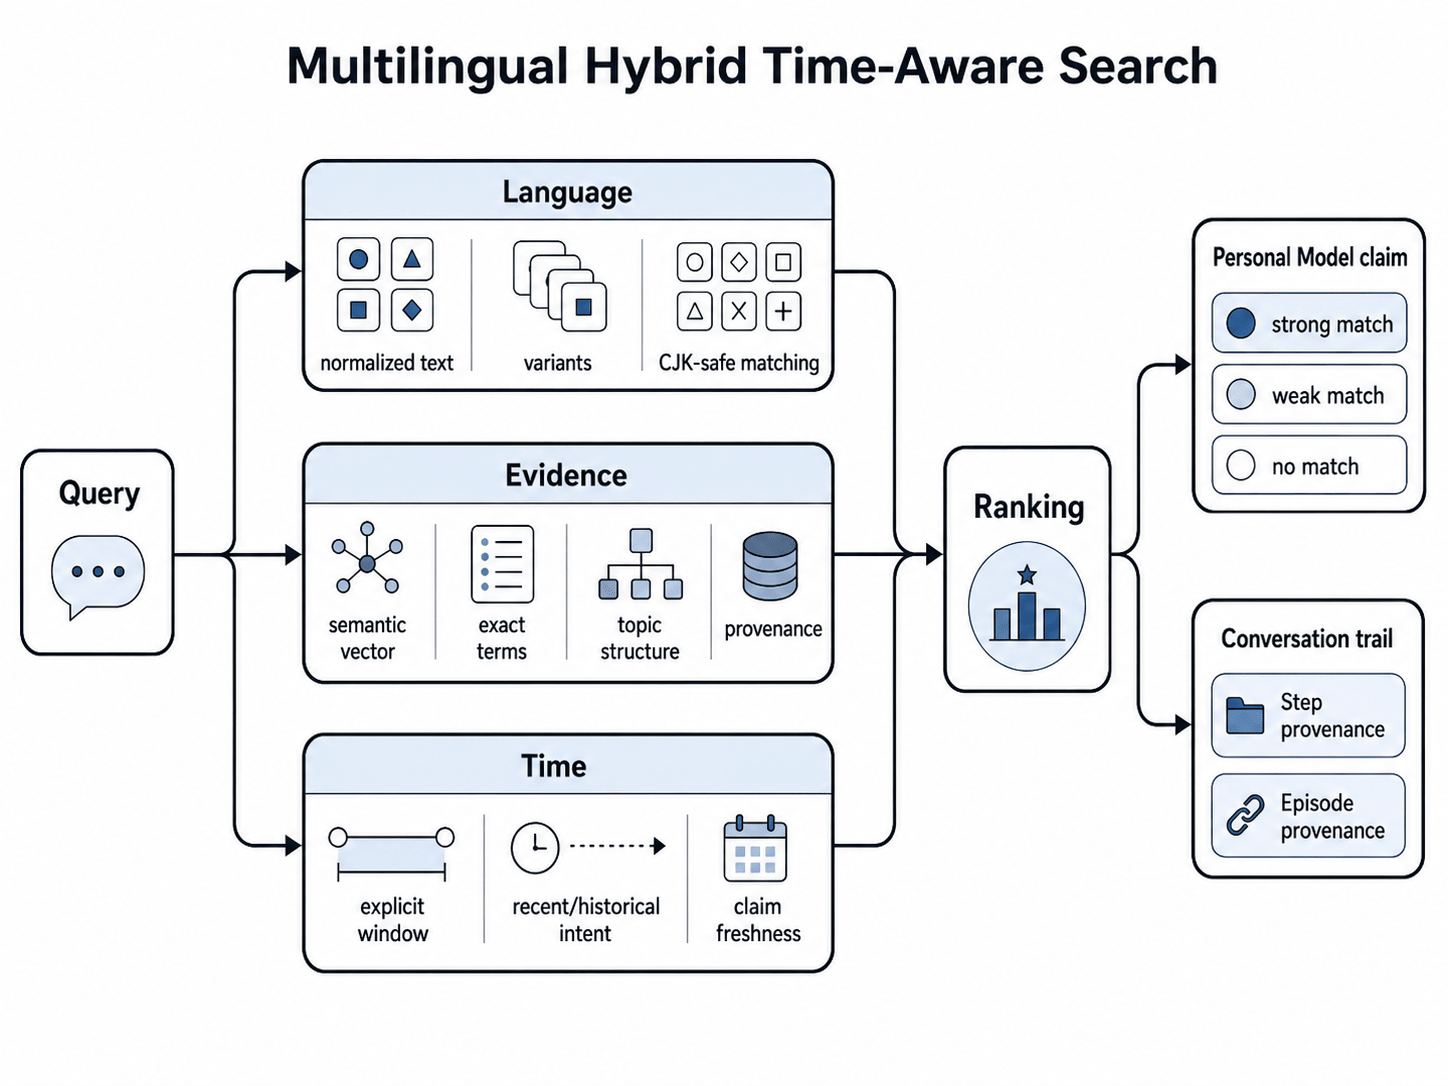
\includegraphics[width=0.9\linewidth]{../../apps/site/static/assets/resources/paper-7.png}
  \caption{Multilingual hybrid time-aware search separates query shaping,
  evidence fusion, and temporal judgment before returning either Personal Model
  claim support or Conversation trail provenance.}
  \label{fig:multilingual-hybrid-time-aware-search}
\end{figure}

\begin{enumerate}[leftmargin=*]
  \item \textbf{Query shaping.} The runtime normalizes Unicode text, preserves
  mixed-language tokens, expands CJK tokens into character n-grams, and accepts
  model-supplied translated or paraphrased \texttt{query\_variants}.
  \item \textbf{Candidate generation.} Hybrid search fuses vector similarity,
  BM25, token coverage, exact keyword matches, and n-gram overlap over the
  scoped semantic index. Personal Model search also adds fielded topic/fact
  matches and source-support text.
  \item \textbf{Time awareness.} Conversation search applies explicit time
  windows and intent-aware recency or historical reranking. Personal Model
  search applies volatility-based freshness so permanent claims remain stable,
  while situational and ephemeral claims lose rank when they have not been used
  recently.
  \item \textbf{Judgment boundary.} Retrieval returns support, not prompt truth.
  Personal Model results are thresholded into \texttt{strong\_match},
  \texttt{weak\_match}, or \texttt{no\_match}; conversation results retain
  Episode, Loop, Step, and source-record provenance.
\end{enumerate}

This lets the system recover a Chinese query over an English thread, or an
English query over a Chinese claim, without relying on a global alias table or
treating nearest-neighbor text as durable understanding.

\subsection{Local Semantic Recall}

Elephant Agent supports a local default embedding path for semantic recall. The local
path lets the user run claim and conversation retrieval without requiring an
external embedding provider. When desired, the embedding provider can be
overridden with a configured remote endpoint and dimensions.

\begin{sloppypar}
The default local provider is \texttt{elephant-local-embed}. It is backed by
\nolinkurl{elephant-embeddings-v1-text-small}, distributed as
\nolinkurl{llm-semantic-router/elephant-embeddings-v1-text-small} on Hugging Face and
\nolinkurl{agentic-intelligence-lab/elephant-embeddings-v1-text-small} on
ModelScope. The runtime loads the model from the local Elephant Agent model root with
\texttt{SentenceTransformer(..., local\_files\_only=True)}.
\end{sloppypar}

The provider exposes three online dimensions: 64, 256, and 768. A lower
dimension gives faster everyday recall; a higher dimension carries more
semantic detail for deeper search. The implementation normalizes vectors and
uses sentence-transformers' truncation path for the selected dimension, so the
same local model can support multiple latency/depth postures.

This is a support-model capability, not the durable truth layer. Embeddings
help find candidate Steps or Facts. The final Personal Model truth remains the
active fact with its status, lens, topic, confidence, and source Episode ids.

\subsection{Background Reflect}

Background reflect is a feature-composable agent system. A trigger fires, a
feature set is resolved, the runner composes a prompt and tools, the sub-agent
receives an evidence packet built from Episode Steps, and the agent calls
tools directly:

\begin{center}
\texttt{episode\_close -> pm/questions/recall -> personal\_model.update}
\end{center}

Feature groups include:

\begin{itemize}[leftmargin=*]
  \item \texttt{pm}: search and write Personal Model facts;
  \item \texttt{questions}: create, settle, or dismiss questions;
  \item \texttt{recall}: search conversation history for support;
  \item \texttt{diary}: write reflective daily entries;
  \item \texttt{skills}: audit visible skill fit without creating hidden
  Personal Model truth;
  \item \texttt{compress}: check compressed content for data loss.
\end{itemize}

Reflect does not use intermediate observations, proposals, or groundings. It
reads Steps directly, writes facts or questions directly through tools, and
persists its run summary in \texttt{learning\_jobs.result\_json}.

\subsection{Deletion, Correction, and Repair}

Durable understanding increases the need for repair. Elephant Agent treats correction as
a normal operation, not an exceptional failure. Corrections can retire active
facts, dispute claims until the user clarifies them, or replace an older fact
for the same lens/topic.

Persistence is valuable only when the user can inspect and correct what
persists. Elephant Agent therefore treats repair paths as part of the runtime contract.
